\lettrine[lhang=0.17]{M}{ost constructions in} category theory are generalizations of results
from other more specific areas of mathematics. Things like products,
coproducts, monoids, exponentials, etc., have been known long before
category theory. They might have been known under different names in
different branches of mathematics. A cartesian product in set theory, a
meet in order theory, a conjunction in logic --- they are all specific
examples of the abstract idea of a categorical product.

The Yoneda lemma stands out in this respect as a sweeping statement
about categories in general with little or no precedent in other
branches of mathematics. Some say that its closest analog is Cayley's
theorem in group theory (every group is isomorphic to a permutation
group of some set).

The setting for the Yoneda lemma is an arbitrary category $\cat{C}$
together with a functor $F$ from $\cat{C}$ to $\Set$. We've
seen in the previous section that some $\Set$-valued functors are
representable, that is isomorphic to a hom-functor. The Yoneda lemma
tells us that all $\Set$-valued functors can be obtained from
hom-functors through natural transformations, and it explicitly
enumerates all such transformations.

When I talked about natural transformations, I mentioned that the
naturality condition can be quite restrictive. When you define a
component of a natural transformation at one object, naturality may be
strong enough to ``transport'' this component to another object that is
connected to it through a morphism. The more arrows between objects in
the source and the target categories there are, the more constraints you
have for transporting the components of natural transformations.
$\Set$ happens to be a very arrow-rich category.

The Yoneda lemma tells us that a natural transformation between a
hom-functor and any other functor $F$ is completely determined by
specifying the value of its single component at just one point! The rest
of the natural transformation just follows from naturality conditions.

So let's review the naturality condition between the two functors
involved in the Yoneda lemma. The first functor is the hom-functor. It
maps any object $x$ in $\cat{C}$ to the set of morphisms
$\cat{C}(a, x)$ --- for $a$ a fixed object in $\cat{C}$. We've
also seen that it maps any morphism $f$ from $x \to y$ to $\cat{C}(a, f)$.

The second functor is an arbitrary $\Set$-valued functor
$F$.

Let's call the natural transformation between these two functors
$\alpha$. Because we are operating in $\Set$, the components of
the natural transformation, like $\alpha_x$ or $\alpha_y$, are just
regular functions between sets:
\begin{gather*}
\alpha_x \Colon \cat{C}(a, x) \to F x \\
\alpha_y \Colon \cat{C}(a, y) \to F y
\end{gather*}

\begin{figure}[H]
\centering
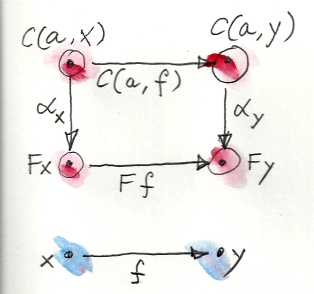
\includegraphics[width=2.73958in]{images/yoneda1.png}
\end{figure}

\noindent
And because these are just functions, we can look at their values at
specific points. But what's a point in the set $\cat{C}(a, x)$? Here's
the key observation: Every point in the set $\cat{C}(a, x)$ is also a
morphism $h$ from $a$ to $x$.

So the naturality square for $\alpha$:
\[\alpha_y \circ \cat{C}(a, f) = F f \circ \alpha_x\]
becomes, point-wise, when acting on $h$:
\[\alpha_y (\cat{C}(a, f) h) = (F f) (\alpha_x h)\]
You might recall from the previous section that the action of the
hom-functor $\cat{C}(a,-)$ on a morphism $f$ was defined as
precomposition:
\[\cat{C}(a, f) h = f \circ h\]
which leads to:
\[\alpha_y (f \circ h) = (F f) (\alpha_x h)\]
Just how strong this condition is can be seen by specializing it to the
case of $x = a$.

\begin{figure}[H]
\centering
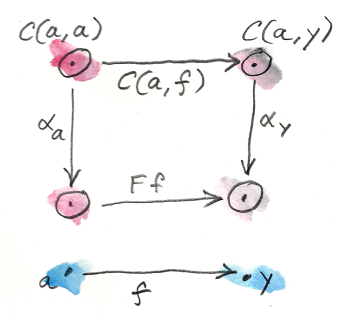
\includegraphics[width=3.12500in]{images/yoneda2.png}
\end{figure}

\noindent
In that case $h$ becomes a morphism from $a$ to
$a$. We know that there is at least one such morphism,
$h = \id_a$. Let's plug it in:
\[\alpha_y f = (F f) (\alpha_a \id_a)\]
Notice what has just happened: The left hand side is the action of
$\alpha_y$ on an arbitrary element $f$ of $\cat{C}(a, y)$. And
it is totally determined by the single value of $\alpha_a$ at
$\id_a$. We can pick any such value and it will generate a natural
transformation. Since the values of $\alpha_a$ are in the set
$F a$, any point in $F a$ will define some $\alpha$.

Conversely, given any natural transformation $\alpha$ from
$\cat{C}(a, -)$ to $F$, you can evaluate it at $\id_a$ to
get a point in $F a$.

We have just proven the Yoneda lemma:

\begin{quote}
There is a one-to-one correspondence between natural transformations
from $\cat{C}(a, -)$ to $F$ and elements of $F a$. 
\end{quote}
in other words,
\[\cat{Nat}(\cat{C}(a, -), F) \cong F a\]
Or, if we use the notation $[\cat{C}, \Set]$ for the functor
category between $\cat{C}$ and $\Set$, the set of natural
transformation is just a hom-set in that category, and we can write:
\[[\cat{C}, \Set](\cat{C}(a, -), F) \cong F a\]
I'll explain later how this correspondence is in fact a natural
isomorphism.

Now let's try to get some intuition about this result. The most amazing
thing is that the whole natural transformation crystallizes from just
one nucleation site: the value we assign to it at $\id_a$. It
spreads from that point following the naturality condition. It floods
the image of $\cat{C}$ in $\Set$. So let's first consider what the
image of $\cat{C}$ is under $\cat{C}(a, -)$.

Let's start with the image of $a$ itself. Under the hom-functor
$\cat{C}(a, -)$, $a$ is mapped to the set $\cat{C}(a, a)$.
Under the functor $F$, on the other hand, it is mapped to the set
$F a$. The component of the natural transformation $\alpha_a$
is some function from $\cat{C}(a, a)$ to $F a$. Let's focus on
just one point in the set $\cat{C}(a, a)$, the point corresponding to
the morphism $\id_a$. To emphasize the fact that it's just a point
in a set, let's call it $p$. The component $\alpha_a$ should map
$p$ to some point $q$ in $F a$. I'll show you that
any choice of $q$ leads to a unique natural transformation.

\begin{figure}[H]
\centering
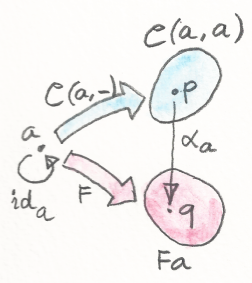
\includegraphics[width=60mm]{images/yoneda3.png}
\end{figure}

\noindent
The first claim is that the choice of one point $q$ uniquely
determines the rest of the function $\alpha_a$. Indeed, let's pick any
other point, $p'$ in $\cat{C}(a, a)$, corresponding to
some morphism $g$ from $a$ to $a$. And here's where
the magic of the Yoneda lemma happens: $g$ can be viewed as a
point $p'$ in the set $\cat{C}(a, a)$. At the same time,
it selects two \emph{functions} between sets. Indeed, under the
hom-functor, the morphism $g$ is mapped to a function
$\cat{C}(a, g)$; and under $F$ it's mapped to $F g$.

\begin{figure}[H]
\centering
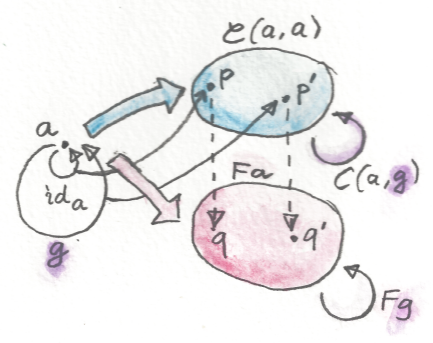
\includegraphics[width=60mm]{images/yoneda4.png}
\end{figure}

\noindent
Now let's consider the action of $\cat{C}(a, g)$ on our original
$p$ which, as you remember, corresponds to $\id_a$. It is
defined as precomposition, $g \circ \id_a$, which is equal to $g$,
which corresponds to our point $p'$. So the morphism
$g$ is mapped to a function that, when acting on $p$
produces $p'$, which is $g$. We have come full
circle!

Now consider the action of $F g$ on $q$. It is some
$q'$, a point in $F a$. To complete the naturality
square, $p'$ must be mapped to $q'$ under
$\alpha_a$. We picked an arbitrary $p'$ (an arbitrary
$g$) and derived its mapping under $\alpha_a$. The function
$\alpha_a$ is thus completely determined.

The second claim is that $\alpha_x$ is uniquely determined for any
object $x$ in $\cat{C}$ that is connected to $a$. The
reasoning is analogous, except that now we have two more sets,
$\cat{C}(a, x)$ and $F x$, and the morphism $g$ from
$a$ to $x$ is mapped, under the hom-functor, to:
\[\cat{C}(a, g) \Colon \cat{C}(a, a) \to \cat{C}(a, x)\]
and under $F$ to:
\[F g \Colon F a \to F x\]
Again, $\cat{C}(a, g)$ acting on our $p$ is given by the
precomposition: $g \circ \id_a$, which corresponds to a point
$p'$ in $\cat{C}(a, x)$. Naturality determines the value
of $\alpha_x$ acting on $p'$ to be:
\[q' = (F g) q\]
Since $p'$ was arbitrary, the whole function $\alpha_x$ is
thus determined.

\begin{figure}[H]
\centering
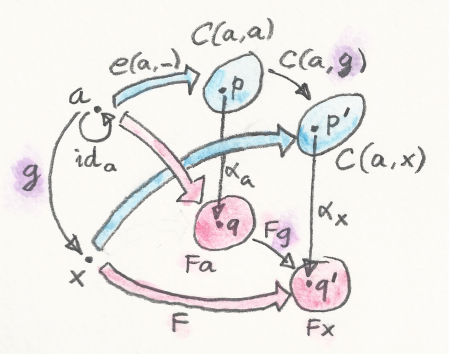
\includegraphics[width=60mm]{images/yoneda5.png}
\end{figure}

\noindent
What if there are objects in $\cat{C}$ that have no connection to
$a$? They are all mapped under $\cat{C}(a, -)$ to a single set
--- the empty set. Recall that the empty set is the initial object in
the category of sets. It means that there is a unique function from this
set to any other set. We called this function \code{absurd}. So here,
again, we have no choice for the component of the natural
transformation: it can only be \code{absurd}.

One way of understanding the Yoneda lemma is to realize that natural
transformations between $\Set$-valued functors are just families
of functions, and functions are in general lossy. A function may
collapse information and it may cover only parts of its codomain. The
only functions that are not lossy are the ones that are invertible ---
the isomorphisms. It follows then that the best structure-preserving
$\Set$-valued functors are the representable ones. They are either
the hom-functors or the functors that are naturally isomorphic to
hom-functors. Any other functor $F$ is obtained from a
hom-functor through a lossy transformation. Such a transformation may
not only lose information, but it may also cover only a small part of
the image of the functor $F$ in $\Set$.

\section{Yoneda in Haskell}

We have already encountered the hom-functor in Haskell under the guise
of the reader functor:

\begin{Verbatim}
type Reader a x = a -> x
\end{Verbatim}
The reader maps morphisms (here, functions) by precomposition:

\begin{Verbatim}
instance Functor (Reader a) where
    fmap f h = f . h
\end{Verbatim}
The Yoneda lemma tells us that the reader functor can be naturally
mapped to any other functor.

A natural transformation is a polymorphic function. So given a functor
\code{F}, we have a mapping to it from the reader functor:

\begin{Verbatim}
alpha :: forall x . (a -> x) -> F x
\end{Verbatim}
As usual, \code{forall} is optional, but I like to write it explicitly
to emphasize parametric polymorphism of natural transformations.

The Yoneda lemma tells us that these natural transformations are in
one-to-one correspondence with the elements of \code{F a}:

\begin{Verbatim}[commandchars=\\\{\}]
forall x . (a -> x) -> F x \ensuremath{\cong} F a
\end{Verbatim}
The right hand side of this identity is what we would normally consider
a data structure. Remember the interpretation of functors as generalized
containers? \code{F a} is a container of \code{a}. But the left
hand side is a polymorphic function that takes a function as an
argument. The Yoneda lemma tells us that the two representations are
equivalent --- they contain the same information.

Another way of saying this is: Give me a polymorphic function of the
type:

\begin{Verbatim}
alpha :: forall x . (a -> x) -> F x
\end{Verbatim}
and I'll produce a container of \code{a}. The trick is the one we used
in the proof of the Yoneda lemma: we call this function with \code{id}
to get an element of \code{F a}:

\begin{Verbatim}
alpha id :: F a
\end{Verbatim}
The converse is also true: Given a value of the type \code{F a}:

\begin{Verbatim}
fa :: F a
\end{Verbatim}
one can define a polymorphic function:

\begin{Verbatim}
alpha h = fmap h fa
\end{Verbatim}
of the correct type. You can easily go back and forth between the two
representations.

The advantage of having multiple representations is that one might be
easier to compose than the other, or that one might be more efficient in
some applications than the other.

The simplest illustration of this principle is the code transformation
that is often used in compiler construction: the continuation passing
style or \acronym{CPS}. It's the simplest application of the Yoneda lemma to the
identity functor. Replacing \code{F} with identity produces:

\begin{Verbatim}[commandchars=\\\{\}]
forall r . (a -> r) -> r \ensuremath{\cong} a
\end{Verbatim}
The interpretation of this formula is that any type \code{a} can be
replaced by a function that takes a ``handler'' for \code{a}. A
handler is a function accepting \code{a} and performing the rest of
the computation --- the continuation. (The type \code{r} usually
encapsulates some kind of status code.)

This style of programming is very common in UIs, in asynchronous
systems, and in concurrent programming. The drawback of \acronym{CPS} is that it
involves inversion of control. The code is split between producers and
consumers (handlers), and is not easily composable. Anybody who's done
any amount of nontrivial web programming is familiar with the nightmare
of spaghetti code from interacting stateful handlers. As we'll see
later, judicious use of functors and monads can restore some
compositional properties of \acronym{CPS}.

\section{Co-Yoneda}

As usual, we get a bonus construction by inverting the direction of
arrows. The Yoneda lemma can be applied to the opposite category
$\cat{C}^{op}$ to give us a mapping between contravariant
functors.

Equivalently, we can derive the co-Yoneda lemma by fixing the target
object of our hom-functors instead of the source. We get the
contravariant hom-functor from $\cat{C}$ to $\Set$:
$\cat{C}(-, a)$. The contravariant version of the Yoneda lemma
establishes one-to-one correspondence between natural transformations
from this functor to any other contravariant functor $F$ and the
elements of the set $F a$:
\[\cat{Nat}(\cat{C}(-, a), F) \cong F a\]
Here's the Haskell version of the co-Yoneda lemma:

\begin{Verbatim}[commandchars=\\\{\}]
forall x . (x -> a) -> F x \ensuremath{\cong} F a
\end{Verbatim}
Notice that in some literature it's the contravariant version that's
called the Yoneda lemma.

\section{Challenges}

\begin{enumerate}
\tightlist
\item
  Show that the two functions \code{phi} and \code{psi} that form
  the Yoneda isomorphism in Haskell are inverses of each other.

\begin{Verbatim}
phi :: (forall x . (a -> x) -> F x) -> F a
phi alpha = alpha id
\end{Verbatim}
\begin{Verbatim}
psi :: F a -> (forall x . (a -> x) -> F x)
psi fa h = fmap h fa
\end{Verbatim}
\item
  A discrete category is one that has objects but no morphisms other
  than identity morphisms. How does the Yoneda lemma work for functors
  from such a category?
\item
  A list of units \code{{[}(){]}} contains no other information but
  its length. So, as a data type, it can be considered an encoding of
  integers. An empty list encodes zero, a singleton \code{{[}(){]}} (a
  value, not a type) encodes one, and so on. Construct another
  representation of this data type using the Yoneda lemma for the list
  functor.
\end{enumerate}

\section{Bibliography}\label{bibliography}

\begin{enumerate}
\tightlist
\item
  \href{https://www.youtube.com/watch?v=TLMxHB19khE}{Catsters} video.\urlfootnote{https://www.youtube.com/watch?v=TLMxHB19khE}
\end{enumerate}